\chapter{Samenvoegbare heaps}
\begin{itemize}
    \item Een samenvoegbare heap is een heap die geoptiamliseerd zijn o mde 'join' operatie uit te voeren.
    \item De join operatie voegt twee heaps samen, zodat de \textbf{heapvoorwaarde} nog steeds geldig is. 
    \item Een lijst van voorbeelden die \underline{niet} gekend moeten zijn (\accentuate{In de cursus is er geen uitleg over \emph{hoe} dat je de samenvoegoperatie zou implementeren voor deze heaps}):
    \begin{itemize}
        \item Leftist tree.
        \item Skew heaps.
        \item Fibonacci heaps.
        \item Relaxed heaps
    \end{itemize}
    
\end{itemize}





De belangrijke samenvoegbare heaps zijn: \textbf{Binomial queues} en \textbf{Pairing heaps}.

\section{Binomiale queues}

		\begin{itemize}
			\item Bestaat uit bos van binomiaalbomen.
			\item Binomiaalboom $B_n$ bestaat uit twee binomiaalbomen $B_{n-1}$. $B_0$ bestaat uit één knoop.
			\item De tweede binomiaalboom is de meest linkse deelboom van de wortel van de eerste.
			\item Een binomiaalboom $B_n$ bestaat uit een wortel met als kinderen $B_{n-1}, ..., B_1, B_0$ (zie figuur \ref{fig:binomialtree_orders})
			\item Op diepte $d$ zijn er $\binom{n}{d}$ knopen.
			\item Voorbeeld: Een prioriteitswachtrij met 13 elementen wordt voorgesteld als $\langle B_3, B_2, B_0 \rangle$.
		\end{itemize}
		\begin{figure}[ht]
			\centering
			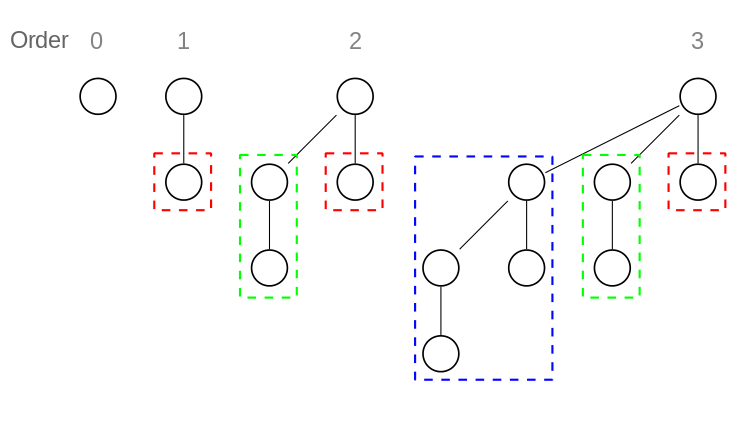
\includegraphics[width=0.75\textwidth]{binomialtree_orders}
			\caption{Verschillende ordes van binomiaalbomen.}
			\label{fig:binomialtree_orders}
		\end{figure}

		De \underline{operaties} op een binomiaalqueue:
		\begin{itemize}
			\item \textbf{Minimum vinden}: Overloop de wortel van elke binomiaalboom. Het minimum kan ook gewoon bijgehouden worden.
			\item \textbf{Samenvoegen}: Tel de bomen met dezelfde hoogte bij elkaar op, $B_h + B_h = B_{h + 1}$. Maak de wortel met de grootste sleutel het kind van deze met de kleinste. 
			\item \textbf{Toevoegen}: Maak een triviale binomiaalqueue met één knoop en voeg deze samen met de andere binomiaalqueue.
			\item \textbf{Minimum verwijderen}: Zoek binomiaalboom $B_k$ met het kleinste wortelelement. Verwijder deze uit de binomiaalqueue. Verwijder wortel van  $B_k$. Voeg beide binomiaalqueues terug samen.
		\end{itemize}

\section{Pairing heaps}
		\begin{itemize}
			\item Een algemene boom waarvan de sleutels voldoen aan de heapvoorwaarde.
			\item Elke knoop heeft een wijzer naar zijn linkerkind en rechterbroer (figuur \ref{fig:pairingheap_treeform} en \ref{fig:pairingheap}). Als verminderen van prioriteit moet ondersteund worden, heeft elke knoop als linkerkind een wijzer naar zijn ouder en als rechterkind een wijzer naar zijn linkerkind.
		\end{itemize}
		\begin{figure}[ht]
			\centering
			\begin{minipage}{.5\textwidth}
				\centering
				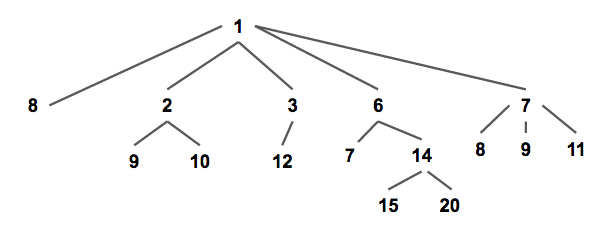
\includegraphics[width=\linewidth]{pairingheap_treeform}
				\caption{Een pairing heap in boomvorm.}
				\label{fig:pairingheap_treeform}
			\end{minipage}%
			\begin{minipage}{.5\textwidth}
				\centering
				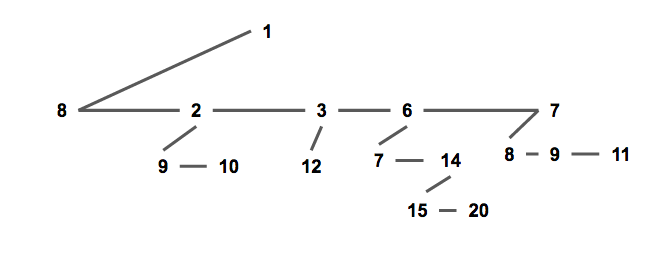
\includegraphics[width=\linewidth]{pairingheap}
				\caption{Een pairing heap.}
				\label{fig:pairingheap}
			\end{minipage}

	
		\end{figure}

		De \underline{operaties} op een pairing heap.
		\begin{itemize}
			\item \textbf{Samenvoegen}: Verlijk het wortelelement van beide heaps. De wortel met het grootste element wordt het linkerkind van deze met het kleinste element.
			\item \textbf{Toevoegen}: Maak een nieuwe pairingheap met één element, en voeg deze samen met de oorspronkelijke heap.
			\item \textbf{Prioriteit wijzigen}: De te wijzigen knoop wordt losgekoppeld, krijgt de prioriteitwijziging, en wordt dan weer samengevoegd met de oorspronkelijke heap.
			\item \textbf{Minimum verwijderen}: De wortel verwijderen levert een collectie van $c$ heaps op. Voeg deze heaps van links naar rechts samen in $O(n)$ of voeg eerst in paren toe, en dan van rechts naar links toevoegen in geamortiseerd $O(\lg n)$.
			\item \textbf{Willekeurige knoop verwijderen}: De te verwijderen knoop wordt losgekoppeld, zodat er twee deelheaps onstaan. Deze twee deelheaps worden samengevoegd.
		\end{itemize}
